\appendix
\chapter*{Eye-To-Hand Calibration Results}
\label{chap:resultsa}


%%%%%%%%%%%%%%%%%
%ASTRA
\begin{figure}[htp]
\begin{center}
{
  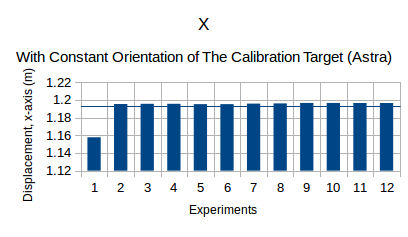
\includegraphics[clip,width=0.5\columnwidth]{figures/constantorientation_astra_x.png}%
}
\end{center}
\begin{center}
{
  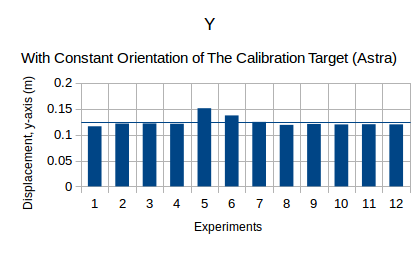
\includegraphics[clip,width=0.5\columnwidth]{figures/constantorientation_astra_y.png}%
}
\end{center}

\begin{center}
{
  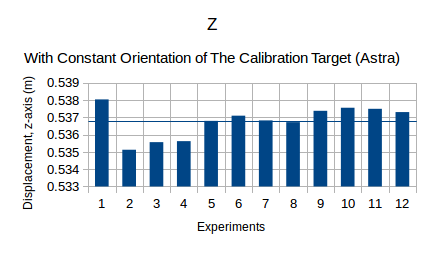
\includegraphics[clip,width=0.5\columnwidth]{figures/constantorientation_astra_z.png}%
}
\end{center}
\caption{Eye-To-Hand Result with a Constant Orientation of the Calibration Plate(Astra Camera)}
\end{figure}

%%%%%%%%%%%%%%%%%%%%
\begin{figure}[htp]
\begin{center}
{
  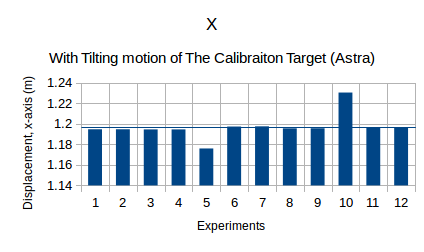
\includegraphics[clip,width=0.5\columnwidth]{figures/tiltingorientation_astra_x.png}%
}
\end{center}
\begin{center}
{
  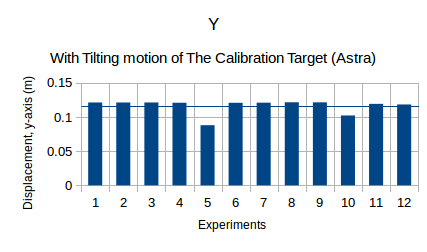
\includegraphics[clip,width=0.5\columnwidth]{figures/tiltingorientation_astra_y.png}%
}
\end{center}

\begin{center}
{
  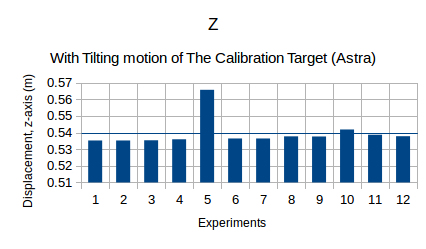
\includegraphics[clip,width=0.5\columnwidth]{figures/tiltingorientation_astra_z.png}%
}
\end{center}
\caption{Eye-To-Hand Result with Tilting Motion of the Calibration Plate(Astra Camera)}
\end{figure}


%%%%%%%%%%%%%%%%%
%REAL


\begin{figure}[htp]
\begin{center}
{
  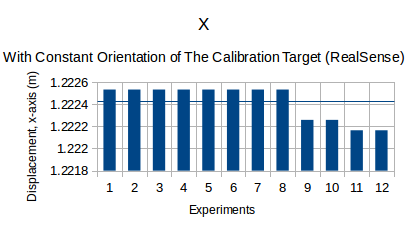
\includegraphics[clip,width=0.5\columnwidth]{figures/constantorientation_real_x.png}%
}
\end{center}
\begin{center}
{
  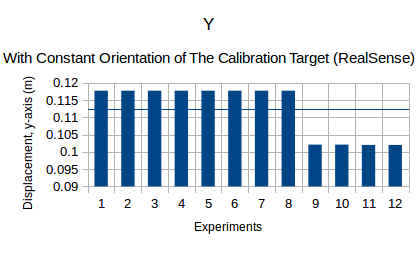
\includegraphics[clip,width=0.5\columnwidth]{figures/constantorientation_real_y.png}%
}
\end{center}

\begin{center}
{
  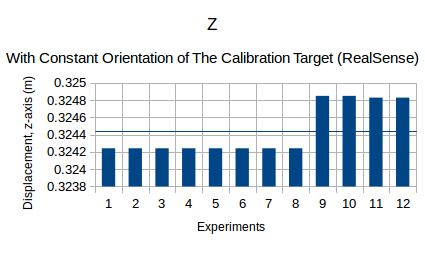
\includegraphics[clip,width=0.5\columnwidth]{figures/constantorientation_real_z.png}%
}
\end{center}
\caption{Eye-To-Hand Result with a Constant Orientation of the Calibration Plate(RealSense)}
\end{figure}

%%%%%%%%%%%%%%%%%%%%
\begin{figure}[htp]
\begin{center}
{
  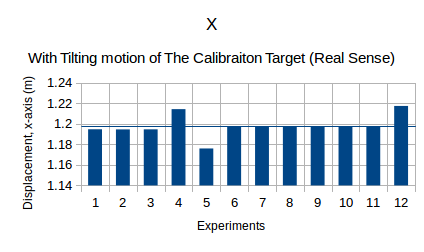
\includegraphics[clip,width=0.5\columnwidth]{figures/tiltingorientation_real_x.png}%
}
\end{center}
\begin{center}
{
  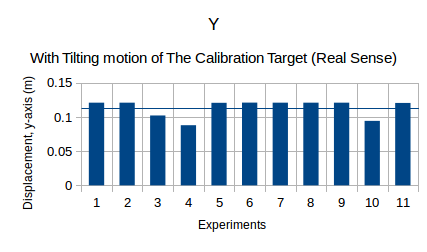
\includegraphics[clip,width=0.5\columnwidth]{figures/tiltingorientation_real_y.png}%
}
\end{center}

\begin{center}
{
  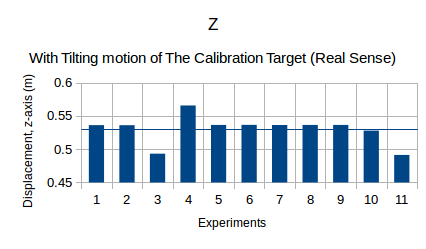
\includegraphics[clip,width=0.5\columnwidth]{figures/tiltingorientation_real_z.png}%
}
\end{center}
\caption{Eye-To-Hand Result with Tilting Motion of the Calibration Plate(RealSense Camera)}
\end{figure}
